\documentclass{article}

\usepackage{iclr2023_conference,times}

\pdfoutput=1

\usepackage{PRIMEarxiv}

\usepackage[utf8]{inputenc} % allow utf-8 input
\usepackage[T1]{fontenc}    % use 8-bit T1 fonts
\usepackage{hyperref}       % hyperlinks
\usepackage{url}            % simple URL typesetting
\usepackage{booktabs}       % professional-quality tables
\usepackage{amsfonts}       % blackboard math symbols
\usepackage{nicefrac}       % compact symbols for 1/2, etc.
\usepackage{microtype}      % microtypography
\usepackage{lipsum}
\usepackage{fancyhdr}       % header
\usepackage{graphicx}       % graphics
\graphicspath{{media/}}     % organize your images and other figures under media/ folder

\usepackage{hyperref}
\usepackage{url}
\usepackage{amsmath}
\usepackage{multirow}
\usepackage{cleveref}
\usepackage{adjustbox}
\usepackage{booktabs}
\usepackage{algorithm2e}
\usepackage{graphicx}

%Header
\pagestyle{fancy}
\thispagestyle{empty}
\rhead{ \textit{ }} 

% Update your Headers here
% \fancyhead[RE]{Firstauthor and Secondauthor} % Firstauthor et al. if more than 2 - must use \documentclass[twoside]{article}



  
%% Title
\title{Augmentation Backdoors}

\author{
  Joseph Rance \\
  University of Cambridge \\
  \texttt{jr879@cam.ac.uk} \\
  %% examples of more authors
   \And
  Yiren Zhao \\
  University of Cambridge \&\\ Imperial College London \\
  \texttt{yiren.zhao@cl.cam.ac.uk} \\
   \And
  Ilia Shumailov \\
  University of Oxford \\
  \texttt{ilia.shumailov@cl.cam.ac.uk} \\
   \And
  Robert Mullins \\
  University of Cambridge \\
  \texttt{Robert.Mullins@cl.cam.ac.uk} \\
  %% \AND
  %% Coauthor \\
  %% Affiliation \\
  %% Address \\
  %% \texttt{email} \\
  %% \And
  %% Coauthor \\
  %% Affiliation \\
  %% Address \\
  %% \texttt{email} \\
  %% \And
  %% Coauthor \\
  %% Affiliation \\
  %% Address \\
  %% \texttt{email} \\
}


\begin{document}
\maketitle
\setcitestyle{authoryear, aysep={,}}

\begin{abstract}
As a popular paradigm for juggling data privacy and collaborative training, federated learning~(FL) is flourishing to distributively process the large scale of heterogeneous datasets on edged clients. Due to bandwidth limitations and security considerations, it ingeniously splits the original problem into multiple subproblems to be solved in parallel, which empowers \textit{primal dual} solutions to great application values in FL. In this paper, we review the recent development of classical \textit{federated primal dual} methods and point out a serious common defect of such methods in non-convex scenarios, which we say is a ``dual drift'' caused by dual hysteresis of those longstanding inactive clients under partial participation training. To further address this problem, we propose a novel \textit{\textbf{A}ligned \textbf{Fed}erated \textbf{P}rimal \textbf{D}ual}~(\textit{\textbf{A-FedPD}}) method, which constructs virtual dual updates to align global consensus and local dual variables for those protracted unparticipated local clients. Meanwhile, we provide a comprehensive analysis of the optimization and generalization efficiency for the \textit{A-FedPD} method on smooth non-convex objectives, which confirms its high efficiency and practicality. Extensive experiments are conducted on several classical FL setups to validate the effectiveness of our proposed method. 
\end{abstract}
%%%%%%%%%%%%%%%%%%%%%%%%%%%%%%%%%%%%%%%%%%%%%%%%%%
\section{Introduction}
\label{main:sec:introduction}
%%%%%%%%%%%%%%%%%%%%%%%%%%%%%%%%%%%%%%%%%%%%%%%%%%

\glsresetall

% \ljh{Just a draft. need polishing and proofreading}
A \gls{np}~\citep{garnelo2018conditional,garnelo2018neural} meta-learns a stochastic process describing the relationship between inputs and outputs in a given data stream, where each task in the data stream consists of a meta-training set of input-output pairs and also a meta-validation set. The \gls{np} then defines an implicit stochastic process whose functional form is determined by a neural network taking the meta-training set as an input, and the parameters of the neural network are optimized to maximize the predictive likelihood for the meta-validation set. This approach is philosophically different from the traditional learning pipeline where one would first elicit a stochastic process from the known class of models (e.g., \glspl{gp}) and hope that it describes the data well. An ideal \gls{np} would assume minimal inductive biases and learn as much as possible from the data. In this regard, \glspl{np} can be framed as a ``data-driven'' way of choosing proper stochastic processes.

 An important design choice for a \gls{np} model is how to capture the uncertainty in the random functions drawn from stochastic processes. When mapping the meta-training set into a function, one might employ a deterministic mapping as in \citet{garnelo2018conditional}. However, it is more natural to assume that there may be multiple plausible functions that might have generated the given data, and thus encode the functional (epistemic) uncertainty as a part of the \gls{np} model. \citet{garnelo2018neural} later proposed to map the meta-training set into a fixed dimensional \emph{global latent variable} with a Gaussian posterior approximation. While this improves upon the vanilla model without such a latent variable~\citep{le2018empirical}, expressing the functional uncertainty only through the Gaussian approximated latent variable has been reported to be a bottleneck~\citep{louizos2019functional}. To this end, \citet{lee2020bootstrapping} and \citet{lee2022neural} propose to apply bootstrap to the meta-training set to use the uncertainty arising from the population distribution as a source for the functional uncertainty.

In this paper, we take a rather different approach to define the functional uncertainty for \glspl{np}. Specifically, we utilize the martingale posterior distribution~\citep{fong2021martingale}, a recently developed alternative to conventional Bayesian inference. In the martingale posterior, instead of eliciting a likelihood-prior pair and inferring the Bayesian posterior, we elicit a joint predictive distribution on future data given observed data. Under suitable conditions on such a predictive distribution, it can be shown that the uncertainty due to the generated future data indeed corresponds to the uncertainty of the Bayesian posterior. Following this, we endow a \gls{np} with a joint predictive distribution defined through neural networks and derive the functional uncertainty as the uncertainty arising when mapping the randomly generated future data to the functions. Compared to the previous approaches of either explicitly positing a finite-dimensional variable encoding the functional uncertainty or deriving it from a population distribution, our method makes minimal assumptions about the predictive distribution and gives more freedom to the model to choose the proper form of uncertainty solely from the data. Due to the theory of martingale posteriors, our model guarantees the existence of the martingale posterior corresponding to the valid Bayesian posterior of an implicitly defined parameter. 
% \ed{Does the following make sense: }
Furthermore, working in the space of future observations allows us to incorporate the latent functional uncertainty path with deterministic path in a more natural manner.
% \ljh{It would be good to have more concrete motivation to prefer the martingale posteriors over conventional Bayesian inference; what would be an advantage of doing that, aside from the fact that we don't need to choose likelihood and prior?} \ed{I'll have a think about this, and will also do some proofreading. Because of the time difference and my job hours, timing might be a bit tricky tomorrow. When would be the best time for me to proofread?}

We name our extension of \glspl{np} with the joint predictive generative models as the \gls{mpnp}. Throughout the paper, we propose an efficient neural network architecture for the generative model that is easy to implement, flexible, and yet guarantees the existence of the martingale posterior. We also propose a training scheme to stably learn the parameters of \glspl{mpnp}. Using various synthetic and real-world regression tasks, we demonstrate that \gls{mpnp} significantly outperforms the previous \gls{np} variants in terms of predictive performance.





% \gls{npf}~\citep{garnelo2018conditional, garnelo2018neural} is a class of parametric models which defines stochastic processes over given data using neural networks.
% Unlike classical stochastic processes (e.g. \glspl{gp}), \gls{npf} learns to fit a proper stochastic processes from data under meta-learning framework.
% The deterministic version of \gls{npf}, \glspl{cnp}~\citep{garnelo2018conditional} deterministically map each dataset to a certain stochastic process which does not consider functional uncertainty.
% In order to compensate for this problem, \glspl{np}~\citep{garnelo2018neural} introduce a global latent variable which captures functional uncertainty.
% \citet{le2018empirical} empirically shows that considering functional uncertainty in \glspl{np} improves the diversity in function realizations and the predictive performance for data.

% Although \glspl{np} tries to capture functional uncertainty, there is some limitations for \glspl{np} to well capture uncertainty with a Gaussian latent variable.
% To overcome this problem, there are some prior works which applying advanced functional uncertainty modeling strategies~\citep{lee2020bootstrapping}\citep{lee2022neural} instead of a global latent variable.
% \gls{bnp}~\citep{lee2020bootstrapping} employs the residual bootstrapping strategy to make more robust uncertainty estimation even for the data-model mismatch situation. 
% However, \gls{bnp} requires a high computational cost compared to \gls{np} due to it's residual bootstrapping strategy.
% \gls{neubnp}~\citep{lee2022neural} employs the recent computationally efficient bootstrapping of the neural network called Neural Bootstrapper~\citep{shin2021neural}.
% However, \gls{neubnp} multiplies Dirichlet distributed random bootstrap weights to features of context dataset which disturbs model to well recovers the given dataset.

% This paper presents a novel extension of \gls{npf} which introduces functional uncertainty by changing posterior uncertainty on function parameters as predictive uncertainty on the unseen data conditional on the observed data...

\section{Related Work}
\label{sec:related work}
\textbf{Communication-efficient training.}
There has been various lines of research focusing on improving communication efficiency in large-scale training, such as using asynchrony \citep{niu2011hogwild,lian2015asynchronous,xie2020zeno++}, decentralization \citep{lian2017can,lu2021optimal}, gradient quantization \citep{alistarh2017qsgd,wen2017terngrad}, gradient sparsification \citep{wangni2017gradient,wang2018atomo}, local steps \citep{stich2018local,lin2018don}, etc. 
In this paper we study the aggressive 1-bit compression, which was first introduced in \citep{seide20141} to speed up speech model training, where an algorithm called 1-bit SGD is proposed. After that, \citet{wen2017terngrad} proposes adding 0 as an additional numerical level and \citet{liu2018signsgd} discusses the use of zero-th order oracle in 1-bit SGD. \citet{chen2019distributed,balles2018dissecting,xu2019signprox} study the correlation and combination between 1-bit SGD and other techniques. Convergence analysis on 1-bit SGD is given in \citep{bernstein2018signsgd,karimireddy2019error,safaryan2021stochastic}. 
\citet{bernstein2018signsgd2,sohn2019election,le2020distributed,lyu2021dp} investigate the robustness of 1-bit SGD.
Among all the variants of 1-bit communication, the design with error feedback mechanism has shown to work best both empirically \citep{seide20141} and theoretically \citep{karimireddy2019error}.
Other lines of research applies 1-bit communication to various scenarios such as federated learning \citep{jin2020stochastic,yue2021federated}, decentralized learning \citep{lu2020moniqua,koloskova2019decentralized}, meta learning \citep{fan2021sign}, etc. Perhaps the closest works to this paper are \citep{tang20211,li20211}, which propose using two-stage training to enable 1-bit Adam and 1-bit Lamb, respectively. Different from those two work, 0/1 Adam addresses non-linearity challenges in adaptive optimizers by considering both extreme quantization and local steps. Furthermore, we also study how to apply extreme communication compression on GPT-style models, which to the best our knowledge is still under-explored.  

\textbf{Adaptive learning rate optimizers.}
One of the most popular adaptive optimizers is Adam, which was first introduced in \citep{kingma2014adam}. It uses both first and second moment information of stochastic gradient to perform optimizer steps and has shown significant benefits on training deep learning models. \citet{reddi2019convergence} spots the issue of Adam convergence and provides a variant called AMSGrad while \citet{zaheer2018adaptive} argues the Adam only converges with large batch sizes.
Multiple lines of theoretical study on Adam are given in \citep{fang2019convergence,alacaoglu2020new,defossez2020simple}.
Additionally,
\citet{chen2018convergence,zhou2018convergence,lu2020mixml,danilova2020recent,zou2019sufficient} provide more general analysis on Adam-type optimizers.
Subsequently, other variants of Adam are proposed in \citep{luo2019adaptive,chen2019zo,huang2018nostalgic,wang2019sadam, zhou2018adashift, zhuang2021momentum,zhuang2020adabelief}. 
Unlike these methods, which focus on improving the convergence of generic optimizations for DNN models, our work studies how to maximize the communication efficiency of Adam in large-scale distributed training settings. 

% the communication efficiency of Adam in data-center model training.
% We emphasize there is a major distinction between these previous works and {\myalgo}, as they 
% investigates how to improve Adam statistically while {\myalgo} studies the communication efficiency of Adam in data-center model training.
\section{Methodology}
\label{methodology}

\begin{wraptable}[10]{r}{0.6\linewidth}
\centering
\vspace{-0.85cm}
%\small
%\renewcommand{\arraystretch}{1}
\caption{Notations adopted in this paper.}
\label{tb:notations}
%\begin{sc}
\begin{tabular}{cc}
\toprule
 Symbol & Notations \\ 
\midrule
 $\mathcal{C}$\ /\ $C$ & client set\ /\ size of client set \\
 $\mathcal{P}$\ /\ $P$ & active client set\ /\ size of active client set \\
 $\mathcal{S}_i$\ /\ $S$ & local dataset\ /\ size of local dataset \\
 $\theta$\ /\ $\theta_i$ & global parameters\ /\ local parameters \\
 $\lambda$\ /\ $\lambda_i$ & global dual parameters\ /\ local dual parameters \\
 $T$\ /\ $t$ & training round\ /\ index of training round\\
 $K$\ /\ $k$ & local interval\ /\ index of local interval\\
 $\rho$ & proxy coefficient \\
\bottomrule
\end{tabular}
\end{wraptable}

We first review the \textit{primal dual} methods in FL and demonstrate the ``\textit{dual drift}'' issue. Then, we demonstrate the \textit{A-FedPD} approach to eliminate the ``\textit{dual drift}'' challenge.
Notations are stated in Table~\ref{tb:notations}. Other symbols are defined when they are first introduced. 
%We denote $(\cdot)_{i}^t$ as the corresponding variable $(\cdot)$ at round $t$ on the client $i$. 
We denote $\mathbb{R}$ as the real set and $\mathbb{E}$ as the expectation in the corresponding probability space. Other notations are defined as first stated.


\subsection{Preliminaries}
\textbf{Setups.} In the general and classical federated frameworks, we usually consider the general objective as a finite-sum minimization problem $F(\theta): \mathbb{R}^d\rightarrow \mathbb{R}$,
\begin{equation}
    \small
    \min_\theta F(\theta) = \frac{1}{C}\sum_{i\in\mathcal{C}}F_i(\theta), \quad F_i(\theta)\triangleq \mathbb{E}_{\xi\sim\mathcal{D}_i}f_i(\theta,\xi).
\end{equation}
In each client, there exists a local private data set $\mathcal{S}_i$ which is considered a uniform sampling set of the distribution $\mathcal{D}_i$. In FL setups, $\mathcal{D}_i$ is unknown to others for the privacy protection mechanism. Therefore, we usually consider the local \textit{Empirical Risk Minimization~(ERM)} as:
\begin{equation}
\label{global_objective}
    \small
    \min_\theta f(\theta) = \frac{1}{C}\sum_{i\in\mathcal{C}}f_i(\theta), \quad f_i(\theta)\triangleq \frac{1}{S}\sum_{\xi\in\mathcal{S}_i}f_i(\theta,\xi).
\end{equation}
Our desired optimal solution is $\theta^\star=\arg\min F(\theta)$. However, we can only approximate it on the limited dataset as $\theta_{\mathcal{S}}^\star=\arg\min f(\theta)$, which spontaneously introduces the unavoidable biases on its generalization performance. This is one of the main concerns in the field of the current machine learning community. Motivated by this imminent challenge, we conduct a comprehensive study on the performance of \textit{primal dual}-based algorithms in FL and further propose an improvement to enhance its generalization efficiency and stability performance.

\subsection{\textit{Primal Dual}-family in FL}
\textit{Primal Dual} methods optimize the global objective by decomposing it into several subproblems and iteratively updating local variables incorporated by Lagrangian multipliers~\citep{boyd2011distributed}, which gives it a unique position in solving FL problems. Due to local data privacy, we have to split the global task into several local tasks for optimization on their private dataset. This similarity also provides an adequate foundation for their applications in the FL community. A lot of studies extend it to the general FL framework and achieve considerable success. 

We follow studies~\citep{zhang2021fedpd,durmus2021federated,wang2022fedadmm,gong2022fedadmm,sun2023fedspeed,zhou2023federated,sun2023dynamic,fan2023federated,zhang2024domain} to summarize the original objective Eq.(\ref{global_objective}) as the global consensus reformulation:
\begin{equation}
\label{consensus_objective}
\small
    \min_{\theta,\theta_i} \frac{1}{C}\sum_{i\in\mathcal{C}}f_i(\theta_i), \quad \text{s.t.} \quad \theta_i=\theta, \quad \forall i\in\mathcal{C}.
\end{equation}
By relaxing equality constraints $\theta_i=\theta$, Eq.(\ref{consensus_objective}) is separable across different local clients. \citet{wang2022fedadmm} demonstrate the difference between the solution on the primal problem and dual problem in detail and confirm the equivalence of these two cases in FL. By penalizing the constraint on the local objective $f_i$, we can define the augmented Lagrangian function associated with Eq.(\ref{consensus_objective}) as:
\begin{equation}
\label{lagrangian}
\small
    \mathcal{L} (\theta_i,\theta,\lambda_i) = \frac{1}{C}\sum_{i\in\mathcal{C}}\left[f_i(\theta_i)\!+\!\langle\lambda_i, \theta_i\!-\!\theta\rangle \!+\! \frac{\rho}{2}\Vert\theta_i\!-\!\theta\Vert^2\right],
\end{equation}
where $\rho$ denotes the penalty coefficient. To train the global model, each local client should first minimize the local augmented Lagrangian function and solve for local parameters. Based on updated local parameters, we then update the dual variable to align the Lagrangian function with the consensus constraints. Finally, we minimize the augmented Lagrangian function and solve for the consensus. Objective Eq.(\ref{consensus_objective}) could be solved after multiple alternating updates as:
\begin{eqnarray}
\label{FedPD}
\small
\begin{cases}
\ \theta_i^{t+1} & = \quad \arg\min_{\theta_i} \ \mathcal{L} (\theta_i^t,\theta^t,\lambda_i^t) \quad i\in\mathcal{C}, \\
\ \lambda_i^{t+1} & =\quad \lambda_i^{t} + \rho(\theta_i^{t+1} - \theta^{t}), \\
\ \theta^{t+1} & =\quad \frac{1}{C}\sum_{i\in\mathcal{C}}(\theta_i^{t+1} + \frac{1}{\rho}\lambda_i^{t+1}).\\
\end{cases}
\end{eqnarray}
We then review the classical \textit{federated primal dual} methods.

\textbf{\textit{FedPD}}. \citet{zhang2021fedpd} propose a general federated framework from the primal-dual optimization perspective which can be directly summarized as Eq.(\ref{FedPD}). As an underlying method in the federated \textit{primal dual}-family, it requires all local clients to participate in the training per round, which also significantly reduces communication efficiency.

\textbf{\textit{FedADMM}}. \citet{wang2022fedadmm} extend the theory of the primal-dual optimization in FL and prove the equivalence between \textit{FedDR}~\citep{tran2021feddr} and \textit{FedADMM}. Furthermore, it considers the complete format of composite objective $f(\theta_i) + g(\theta)$. To optimize the composite objective, after the iterations of Eq.(\ref{FedPD}), it additionally solves the proximal step on the function $g(\theta)$:
\begin{eqnarray}
\label{FedADMM}
\small
\begin{cases}
\ \theta_i^{t+1} & = \quad \arg\min_{\theta_i} \ \mathcal{L} (\theta_i^t,\theta^t,\lambda_i^t) + g(\theta^t) \quad i\in\mathcal{P}^t, \\
\ \lambda_i^{t+1} & =\quad \lambda_i^{t} + \rho(\theta_i^{t+1} - \theta^t), \\
\ \overline{\theta}^{t+1} & =\quad \frac{1}{P}\sum_{i\in\mathcal{P}^t}(\theta_i^{t+1} + \frac{1}{\rho}\lambda_i^{t+1}), \\
\ \theta^{t+1} &=\quad \arg\min g(\theta^t) + \frac{1}{2\rho}\Vert \theta^t -\overline{\theta}^{t+1} \Vert^2.\\
\end{cases}
\end{eqnarray}
\textit{FedADMM} introduces a more general update with the regularization term $g(\theta)$ and supports the partial participation training mechanism, which also brings a great application value of primal-dual methods to the FL community. When $g(\cdot)\equiv 0$, it degrades to the partial \textit{FedPD} by $\theta^{t+1} = \overline{\theta}^{t+1}$. When $\mathcal{P}^t\neq\mathcal{C}$, ``\textit{dual drift}'' brings great distress for training.

\textbf{\textit{FedDyn}}. \citet{durmus2021federated} utilize the insight of primal-dual optimization to introduce a dynamic regularization term to solve the local augmented Lagrangian function, which is actually the dual variable in \textit{FedADMM}. Differently, they propose a global dual variable $\lambda^t$ to update global parameters $\theta^t$ instead of only active local dual variables $\lambda_i^t$~($i\in\mathcal{P}^t$):
\begin{eqnarray}
\label{FedDyn}
\small
\begin{cases}
\ \theta_i^{t+1} & = \quad \arg\min_{\theta_i} \ \mathcal{L} (\theta_i^t,\theta^t,\lambda_i^t) \quad i\in\mathcal{P}^t, \\
\ \lambda_i^{t+1} & =\quad \lambda_i^{t} + \rho(\theta_i^{t+1} - \theta^t), \\
\ \lambda^{t+1} &=\quad \lambda^{t} + \rho\frac{1}{C}\sum_{i\in\mathcal{P}^t}(\theta_i^{t+1} - \theta^t), \\
\ \theta^{t+1} &=\quad \frac{1}{P}\sum_{i\in\mathcal{P}^t}\theta_i^{t+1} + \frac{1}{\rho}\lambda^t.\\
\end{cases}
\end{eqnarray}
Compared with \textit{FedADMM}, although the global dual variable further corrects the primal parameters, it still hinders the training efficiency, which must rely on the anachronistic historical directions of the local dual variables. Moreover, the global dual variable always updates slowly, which results in consensus constraints that are more difficult to satisfy when solving local subproblems.

\textbf{\textit{Dual drift}}. \citet{kang2024fedand} have indicated that the update mismatch between primal and dual variables leads to a ''drift''. Here, we provide a detailed analysis of the key differences caused by this mismatch. When adopting partial participation, each client is activated at a very low probability, especially on a large scale of edged devices, which widely leads to very high hysteresis between global parameters $\theta$ and local dual variable $\lambda_i$. For instance, at round $t$, we select a subset $\mathcal{P}^t$ to participate in current training and then update the global parameters by $\theta^{t+1} = \arg\min_{\theta} \ \mathcal{L} (\theta_i^{t+1},\theta^t,\lambda_i^t)$ for $i\in\mathcal{P}^t$. Then at round $t+1$, when a client $i\notin \{\mathcal{P}^\tau\}_{\tau=t_0+1}^{t}$~$(t_0\ll t)$ that has not been involved in training for a long time is activated, its local dual variable $\lambda_i^{t_0}$ may severely mismatch the current global parameters $\theta^t$. This triggers that the local subproblem $\mathcal{L} (\theta_i^{t+1},\theta^{t+1},\lambda_i^{t_0})$ fail to be optimized properly and even become completely distorted in extreme scenarios, yielding a ``\textit{dual drift}'' issue. 

\subsection{A-FedPD Method}

As introduced in the last part, ``\textit{dual drift}'' problem usually results in the unstable optimization of each local subproblem under partial participation.
To further mitigate the negative effects of \textit{dual drift} problems and improve the training efficiency, we propose a novel \textit{A-FedPD} method (see Algorithm \ref{algorithm:dual_update}), which aligns the virtual dual variables of unparticipated clients via global average models.

Specifically, we solve dual variables for unified management and distribution. At round $t$, we select an active client set $\mathcal{P}^t$ and send the corresponding variables to each active client. Then local client solves the subproblem with $K$ stochastic gradient descent steps and sends the last state $\theta_{i,K}^t$ back to the global server. On the global server, it first aggregates the updated parameters as $\overline{\theta}^{t+1}$. Then it performs the updates of the dual variables. For each active client $i\in\mathcal{P}^t$, it equally updates the local dual variable as vanilla \textit{FedPD}. For the unparticipated clients $i\notin \mathcal{P}^t$, they update the virtual dual variable with the aggregated parameters $\overline{\theta}^{t+1}$. Finally, we can update the global model with the aggregated parameters and averaged dual variables. Since each client virtually updates, we can directly use the global average as the output. Repeat this training process for a total of $T$ communication rounds to output the final global average model. 

\begin{algorithm}[t]
\small
	\renewcommand{\algorithmicrequire}{\textbf{Input:}}
	\renewcommand{\algorithmicensure}{\textbf{Output:}}
	\caption{A-FedPD Algorithm}
    \begin{multicols}{2}
	\begin{algorithmic}[1]
		\REQUIRE $\theta^0$, $\theta_i^0$, $T$, $K$, $\lambda_i^0$, $\rho$
		\ENSURE global average model\\
            \STATE \textbf{Initialization} : $\theta_i^0=\theta^0$, $\lambda_i^0=0$.
            \FOR{$t = 0, 1, 2, \cdots, T-1$}
            \STATE randomly select active clients set $\mathcal{P}^t$ from $\mathcal{C}$
            \FOR{client $i \in \mathcal{P}^t$ \textbf{in parallel}}
            \STATE receive $\lambda_i^t, \theta^t$ from the global server
            %\STATE (A2) {\color{red}{$\lambda_i^{t+1} = \lambda_i^t + \rho(w_i^{t+1} - w^t)$}}
            \STATE $\theta_i^{t+1} = \textit{LocalTrain}(\lambda_i^t, \theta^t, \eta^t, K)$
            %\STATE $\lambda_i^{t+1} = \lambda_i^t + \rho(w_i^{t+1} - w^t)$
            \STATE send $\theta_i^{t+1}$ to the global server 
            \ENDFOR
            %\STATE $\lambda^{t+1} = \lambda^t + \frac{1}{C}\sum_{i\in \mathcal{N}^t}\rho(w_{i}^{t+1}-w^t)$
            \STATE $\overline{\theta}^{t+1} = \frac{1}{P}\sum_{i\in\mathcal{P}^t}\theta_i^{t+1}$
            \STATE $\lambda_i^{t+1}=\textit{D-Update}(\lambda_i^t, \theta^t, \theta_i^{t+1}, \overline{\theta}^{t+1}, \mathcal{P}^t)$
            \STATE $\overline{\lambda}^{t+1} = \frac{1}{C}\sum_{i\in\mathcal{C}}\lambda_i^{t+1}$
            \STATE $\theta^{t+1} = \overline{\theta}^{t+1} + \frac{1}{\rho} \overline{\lambda}^{t+1}$
            \ENDFOR
            \STATE return global average model
	\end{algorithmic}
    \label{algorithm}
    \textit{$\diamondsuit$ LocalTrain}: (Optimize Eq.(\ref{lagrangian}))
    \begin{algorithmic}[1]
	\REQUIRE $\lambda_i^t$, $\theta^t$, $\eta^t$, $K$
	\ENSURE $\theta_{i,K}^t$
        \FOR{$k = 0, 1, 2, \cdots, K-1$}
        \STATE calculate the stochastic gradient $g_{i,k}^t$
        \STATE $\theta_{i,k+1}^t = \theta_{i,k}^t - \eta^t(g_{i,k}^t + \lambda_i^t + \rho(\theta_{i,k}^t - \theta^t))$
        \ENDFOR
	\end{algorithmic}
	\label{algorithm:local_update}

    \vspace{0.4cm}
    \textit{$\diamondsuit$ D-Update}:~(update dual variables)
    \begin{algorithmic}[1]
    \REQUIRE $\lambda_i^t, \theta^t, \theta_i^{t+1}, \overline{\theta}^{t+1}, \mathcal{P}^t$
	\ENSURE $\lambda_i^{t+1}$
    \IF{$i\in\mathcal{P}^t$}
    \STATE $\lambda_i^{t+1} = \lambda_i^{t} + \rho_t(\theta_i^{t+1} - \theta^t)$
    \ELSE 
    \STATE $\lambda_i^{t+1} = \lambda_i^{t} + \rho_t(\overline{\theta}^{t+1} - \theta^t)$
    \ENDIF
    \end{algorithmic}
\label{algorithm:dual_update}
\end{multicols}
\vspace{-0.3cm}
\end{algorithm}  

Because of the central storage and management of the dual variables on the global server, it significantly reduces storage requirements for lightweight-edged devices, i.e., mobile phones. For the unparticipated clients, we use their unbiased estimations $\mathbb{E}\left[w_i^{t+1}\vert \ w^{t}\right]=\mathbb{E}_{\mathcal{P}^t}\left[\frac{1}{P}\sum_{i\in\mathcal{P}^t}w_i^{t+1}\vert \ w^{t}\right]$ to construct the virtual dual update, which maintains a continuous update of local dual variables. For the global averaged dual variable $\overline{\lambda}$, we can reformulate its update as $\overline{\lambda}^{t+1}=\overline{\lambda}^t + \rho(\overline{\theta}^{t+1} - \theta^t)$ which also could be approximated as a virtual all participation case. This efficiently alleviates the \textit{dual drift} between $\theta^t$ and $\lambda_i^t$ and also ensures fast iteration of the global dual variable in the training, which constitutes an efficient federated framework. 

% \textbf{\textit{Diminished biases.}} The true dual update of each local client is $\lambda_i^{t+1} = \lambda_i^t + \rho(\theta_i^{t+1} - \theta^t)$. The gap between the true update and our virtual update is $\rho(\theta_i^{t+1} - \overline{\theta}^{t+1})$. When the local subproblem is well solved under $t\rightarrow\infty$, as analyzed by \citet{durmus2021federated}, the local objective aligns with the global one, which implies $\sum_i\nabla f_i(\theta_i^\infty)\rightarrow\sum_i\nabla f_i(\theta^\infty)=0$. Then $\theta_i^\infty\rightarrow\theta^\infty\rightarrow\overline{\theta}^{\infty}$ as local dual variables are also well solved to zero. Final estimation bias decreases as optimization goes and diminishes to a very low value, which aligns with the global consensus.



\section{Evaluation} \label{eval}

% To evaluate the effectiveness of each component in our algorithm design, we introduce three variants of our algorithm: BA-MBRL, BA-MCTS, and BA-MCTS-SL. (1) Existing offline MBRL methods leverage learned world models as surrogate simulators, applying reward penalties to collected transitions and employing standard online RL algorithms (e.g., SAC (\cite{DBLP:conf/icml/HaarnojaZAL18})) to learn a policy. BA-MBRL follows this approach but models the problem as a BAMDP, with environment transitions defined by Equations (\ref{bamdp-mdp}) and (\ref{b'}) and the reward penalty given by Equation (\ref{p-rwd}). BA-MBRL is designed to evaluate the effectiveness of Bayesian RL. (2) Building on BA-MBRL, BA-MCTS introduces Continuous BAMCP (Algorithm \ref{alg:2}) to plan at decision points, rather than inferring directly from the policy, to generate trajectories for downstream SAC. BA-MCTS demonstrates the impact of deep search on policy learning. (3) BA-MCTS-SL, described in Algorithm \ref{alg:3}, replaces the policy learning algorithm in BA-MCTS from policy gradient methods (as in SAC) with supervised learning (SL). By comparing these two approaches, we aim to determine which method offers a more efficient policy update mechanism, particularly for continuous control tasks.

To evaluate the effectiveness of each component in our algorithm design, we introduce three variants: (1) \textbf{BA-MBRL} leverages learned world models as surrogate simulators, applying reward penalties to collected transitions and using standard online RL algorithms (e.g., SAC (\cite{DBLP:conf/icml/HaarnojaZAL18})) to learn a policy. While following existing offline MBRL methods, it models the problem as a BAMDP (rather than an MDP), with environment transitions defined by Equations (\ref{bamdp-mdp}) and (\ref{b'}) and the reward penalty by Equation (\ref{p-rwd}), and is designed to evaluate the effectiveness of Bayesian RL. (2) \textbf{BA-MCTS} builds on BA-MBRL by introducing Continuous BAMCP (Algorithm \ref{alg:2}) to plan at decision points, rather than inferring directly from the policy, to generate trajectories for downstream SAC, demonstrating the impact of deep search on policy learning. (3) \textbf{BA-MCTS-SL}, described in Algorithm \ref{alg:3}, replaces the policy learning algorithm in BA-MCTS from policy gradient methods (as in SAC) with supervised learning (SL), allowing us to compare which approach offers a more efficient policy update mechanism, particularly for continuous control tasks.
 
\begin{table}[t]
\scriptsize
\centering
\begin{tabular}{c|c|c|c|c|c|c|c|c}
\hline
{\makecell{Data Type}} & {Environment} & {\makecell{BA-MCTS \\ -SL (ours)}} & {\makecell{BA-MCTS \\ (ours)}} & {\makecell{BA-MBRL \\ (ours)}} & {Optimized} & {COMBO} & {MOReL} & {MOPO}\\
\hline 
\hline
{random} & {HalfCheetah} & {29.20 $\pm$ 2.00} & {36.23 $\pm$ 1.04} & {32.76 $\pm$ 1.16} & {31.7} & {\textbf{38.8}} & {25.6} & {35.4} \\
{random} & {Hopper} & {33.83 $\pm$ 0.10} & {31.56 $\pm$ 0.12} & {31.47 $\pm$ 0.03} & {12.1} & {17.9} & {\textbf{53.6}} & {11.7} \\
{random} & {Walker2d} & {21.89 $\pm$ 0.07} & {21.59 $\pm$ 0.32} & {21.45 $\pm$ 0.53} & {21.7} & {7.0} & {\textbf{37.3}} & {13.6} \\
\hline
{medium} & {HalfCheetah} & {70.47 $\pm$ 3.52} & {\textbf{75.84} $\pm$ 3.81} & {56.54 $\pm$ 5.20} & {45.7} & {54.2} & {42.1} & {42.3} \\
{medium} & {Hopper} & {97.75 $\pm$ 7.09} & {96.70 $\pm$ 14.0} & {\textbf{98.25} $\pm$ 3.42} & {69.3} & {97.2} & {95.4} & {28.0} \\
{medium} & {Walker2d} & {\textbf{82.24} $\pm$ 1.85} & {74.73 $\pm$ 3.25} & {75.41 $\pm$ 4.17} & {79.7} & {81.9} & {77.8} & {17.8} \\
\hline 
{med-replay} & {HalfCheetah} & {61.16 $\pm$ 1.60} & {\textbf{65.45} $\pm$ 0.81} & {62.50 $\pm$ 0.18} & {58.0} & {55.1} & {40.2} & {53.1} \\
{med-replay} & {Hopper} & {\textbf{106.3} $\pm$ 0.13} & {101.8 $\pm$ 3.46} & {93.91 $\pm$ 4.25} & {90.8} & {89.5} & {93.6} & {67.5} \\
{med-replay} & {Walker2d} & {92.13 $\pm$ 5.13} & {95.06 $\pm$ 2.11} & {\textbf{97.54}$\pm$ 1.93} & {65.8} & {56.0} & {49.8} & {39.0} \\
\hline 
{med-expert} & {HalfCheetah} & {80.53 $\pm$ 6.63} & {76.16 $\pm$ 10.3} & {90.52 $\pm$ 4.13} & {\textbf{104.2}} & {90.0} & {53.3} & {63.3} \\
{med-expert} & {Hopper} & {\textbf{112.2} $\pm$ 0.29} & {108.3 $\pm$ 0.22} & {107.8 $\pm$ 0.37} & {105.8} & {111.1} & {108.7} & {23.7} \\
{med-expert} & {Walker2d} & {107.7 $\pm$ 0.82} & {\textbf{110.0} $\pm$ 1.74} & {84.71 $\pm$ 0.87} & {97.1} & {103.3} & {95.6} & {44.6} \\
\hline
\hline
\multicolumn{2}{c|}{Average Score} & {\textbf{74.62}} & {74.45} & {71.06} & {65.16} & {66.83} & {64.42} & {36.67} \\
\hline 
\end{tabular}
\caption{Comparisons between the proposed algorithms and SOTA offline model-based RL methods on the D4RL benchmark suite. Each value represents the normalized score, as proposed in (\cite{DBLP:journals/corr/abs-2004-07219}), of the policy trained by the corresponding algorithm. These scores are undiscounted returns normalized to approximately range between 0 and 100, where a score of 0 corresponds to a random policy and a score of 100 corresponds to an expert-level policy. For our algorithms, we report the average score of the final ten policy learning epochs and its standard deviation across three random seeds. Results in the last four columns are taken from the original papers (\cite{DBLP:conf/iclr/LuBPOR22, DBLP:conf/nips/YuKRRLF21, DBLP:conf/nips/KidambiRNJ20, DBLP:conf/nips/YuTYEZLFM20}), respectively.} 
\label{table:1}
\end{table}

We first evaluate our algorithms on a widely-used continuous control benchmark for offline RL methods -- D4RL MuJoCo (\cite{DBLP:journals/corr/abs-2004-07219}). The evaluation results for three types of robotic agents, each with offline datasets of four different qualities, are presented in Table \ref{table:1}. (1) Compared to SOTA offline MBRL methods, our algorithms achieve superior performance on nine out of twelve tasks. In terms of average performance, BA-MBRL significantly outperforms the baselines, demonstrating the effectiveness of using BAMDPs to handle model uncertainties in offline MBRL. (2) Both BA-MCTS and BA-MCTS-SL further improve upon BA-MBRL, highlighting the enhancement brought by deep search in policy learning. Notably, we apply Continuous BAMCP to only 10\% of states when collecting training trajectories, while for the remaining states, we sample actions directly from the policy, i.e., $a \sim \pi(\cdot|s)$. Increasing the search ratio could further enhance policy performance at the cost of increased computation. (3) BA-MCTS-SL performs similarly to BA-MCTS, validating the effectiveness of both policy update mechanisms. However, BA-MCTS-SL struggles on Walker2d, where a warm-up training phase (using BA-MBRL) is required to establish a better initial policy. On the other hand, the advantage of the SL-based policy update is evident in the training plots of our algorithms in Figure \ref{fig:3}, where BA-MCTS-SL exhibits much smoother learning curves compared to the other two algorithms, indicating greater robustness in model selection. (4) We further compare our algorithms with model-free offline policy learning methods, as shown in Appendix \ref{ComMF}. The performance improvement is even greater than that over model-based methods, highlighting the necessity of model-based learning. Particularly, when data quality is low, merely mimicking or staying close to the behavior policy would result in an underperforming policy. (5) We provide an ablation study in Appendix \ref{ASRP} to demonstrate the necessity of incorporating the reward penalty in offline MBRL to prevent the overexploitation of inaccurate world models. Additionally, we find that the SL-based policy update is less sensitive to model inaccuracies.

\begin{figure*}[t]
\centering
\subfigure[hc-med-expert]{
\label{fig:1(a)} 
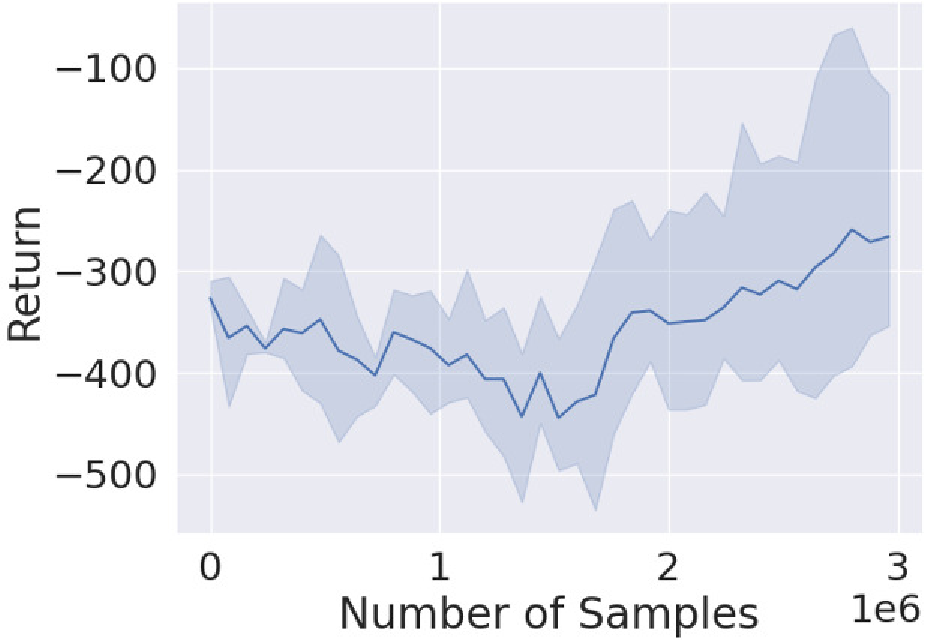
\includegraphics[width=1.5in, height=0.8in]{hc-m-exp-mz.pdf}}
\subfigure[hc-med-replay]{
\label{fig:1(b)} 
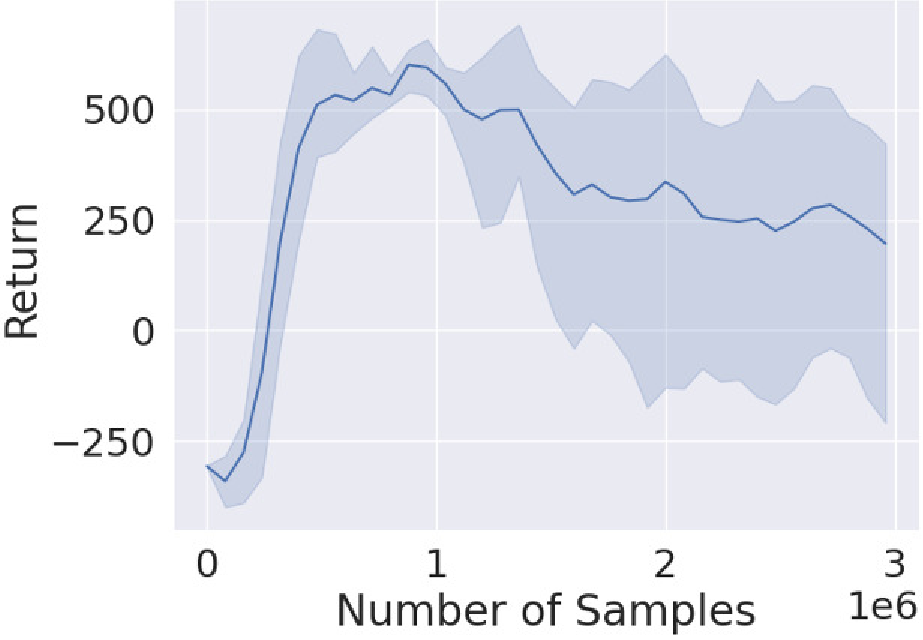
\includegraphics[width=1.5in, height=0.8in]{hc-m-rep-mz.pdf}}
\subfigure[hc-medium]{
\label{fig:1(c)} 
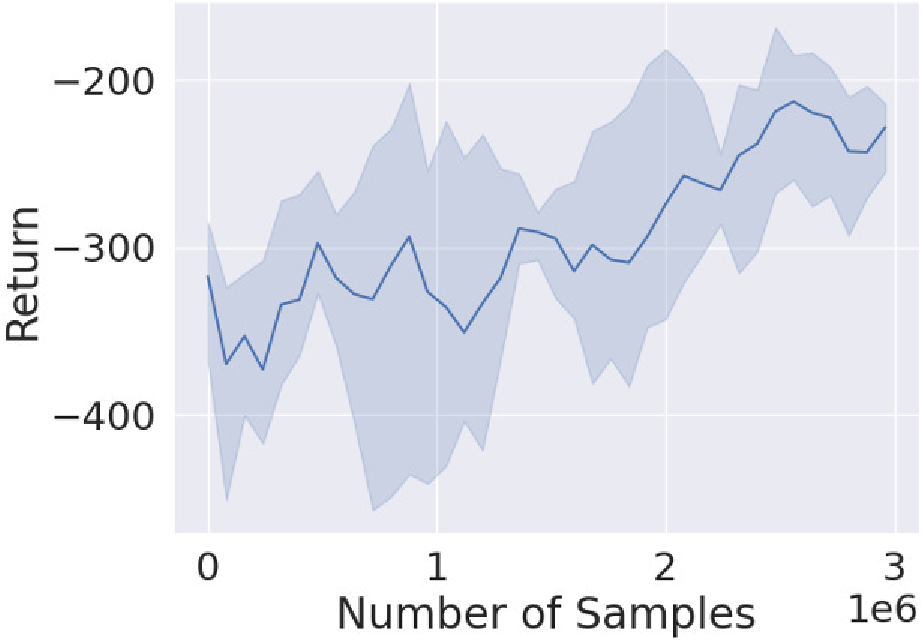
\includegraphics[width=1.5in, height=0.8in]{hc-med-mz.pdf}}
\subfigure[hc-random]{
\label{fig:1(d)} 
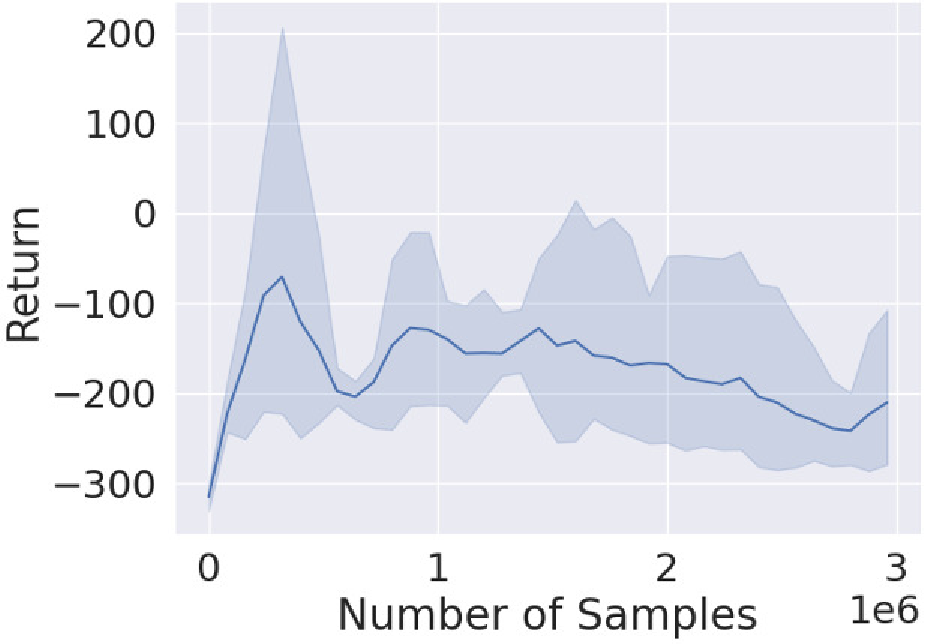
\includegraphics[width=1.5in, height=0.8in]{hc-rnd-mz.pdf}}
\subfigure[hp-med-expert]{
\label{fig:1(e)} 
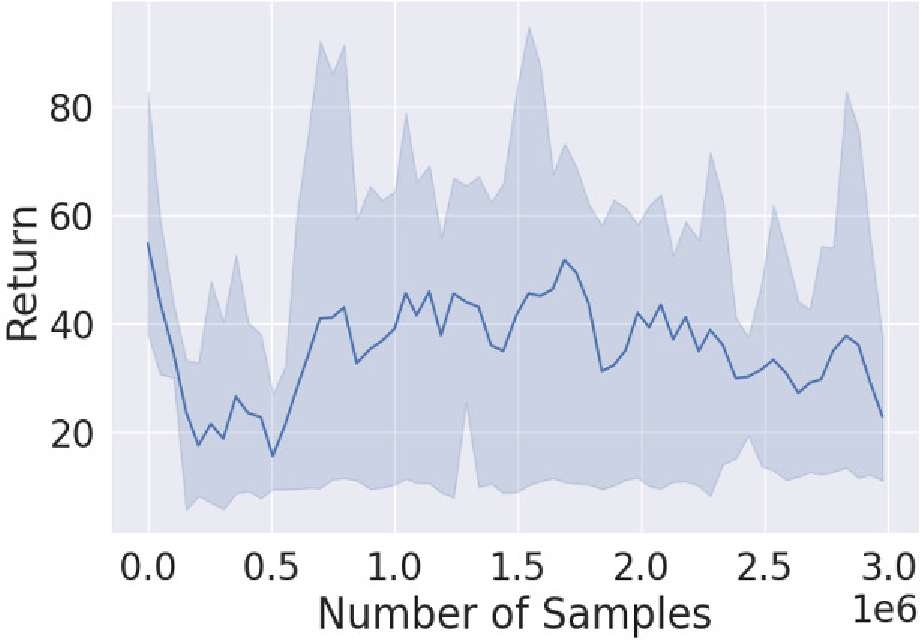
\includegraphics[width=1.5in, height=0.8in]{hp-m-exp-mz.pdf}}
\subfigure[hp-med-replay]{
\label{fig:1(f)} 
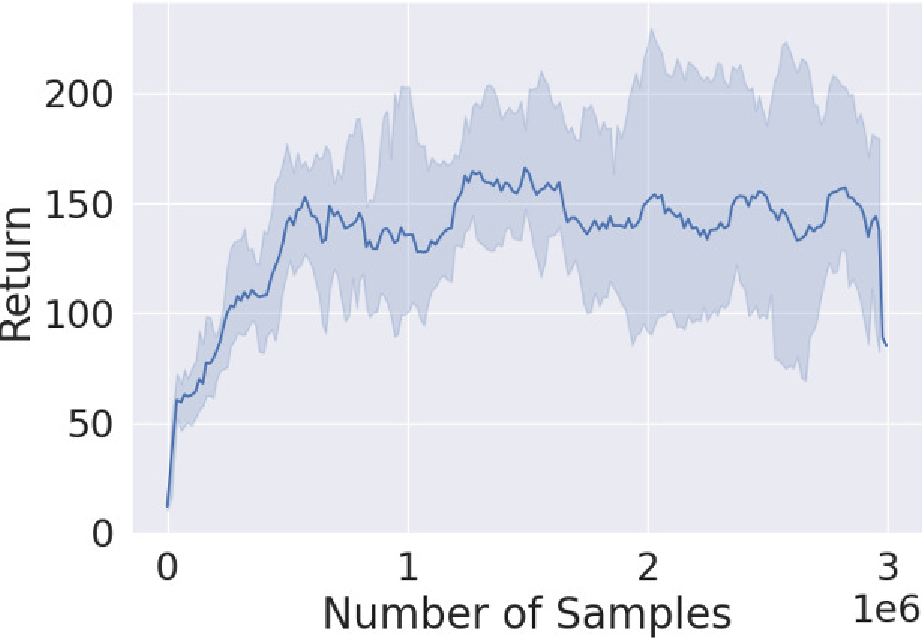
\includegraphics[width=1.5in, height=0.8in]{hp-m-rep-mz.pdf}}
\subfigure[hp-medium]{
\label{fig:1(g)} 
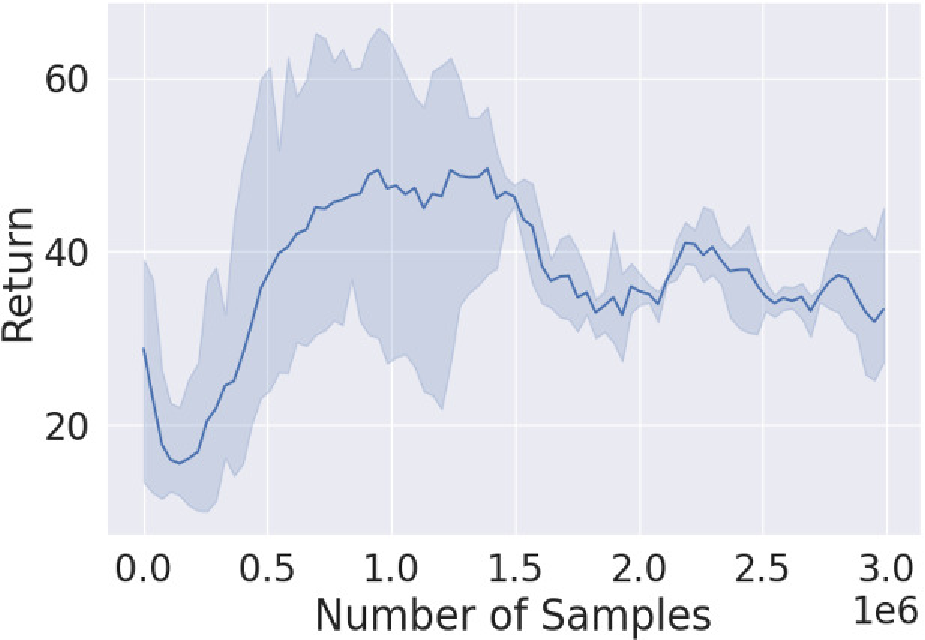
\includegraphics[width=1.5in, height=0.8in]{hp-med-mz.pdf}}
\subfigure[hp-random]{
\label{fig:1(h)} 
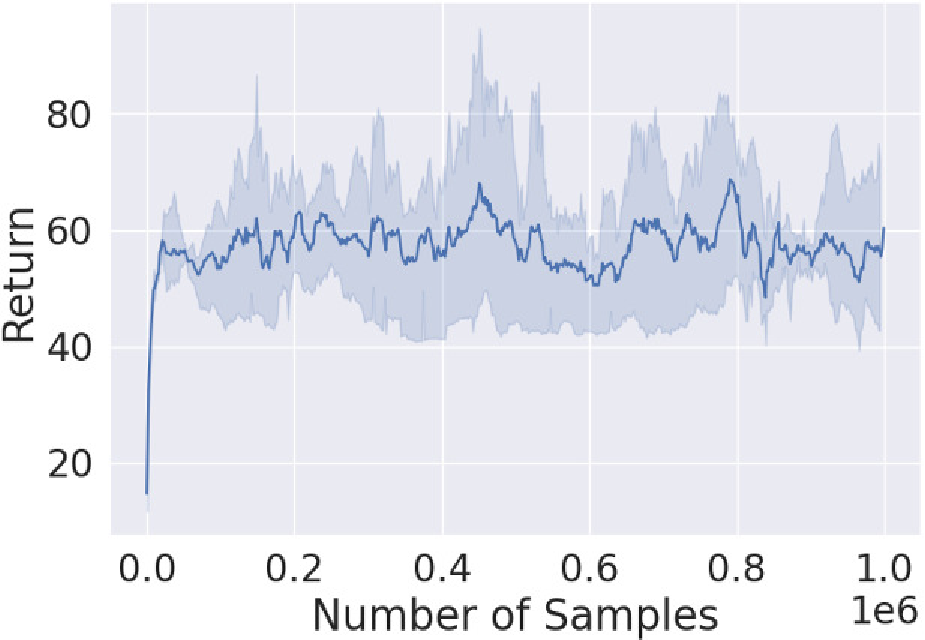
\includegraphics[width=1.5in, height=0.8in]{hp-rnd-mz.pdf}}
\subfigure[wk-med-expert]{
\label{fig:1(i)} 
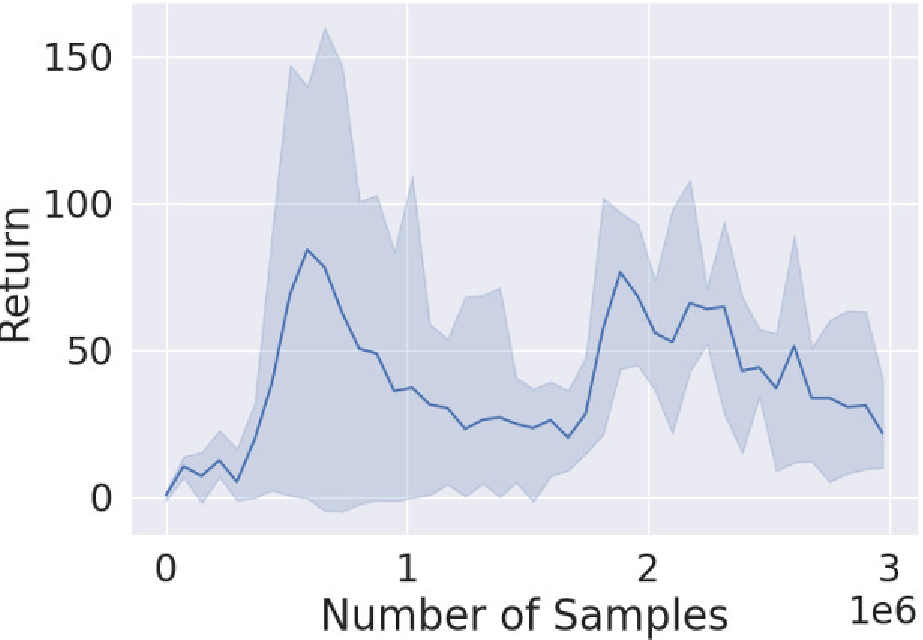
\includegraphics[width=1.5in, height=0.8in]{wk-m-exp-mz.pdf}}
\subfigure[wk-med-replay]{
\label{fig:1(j)} 
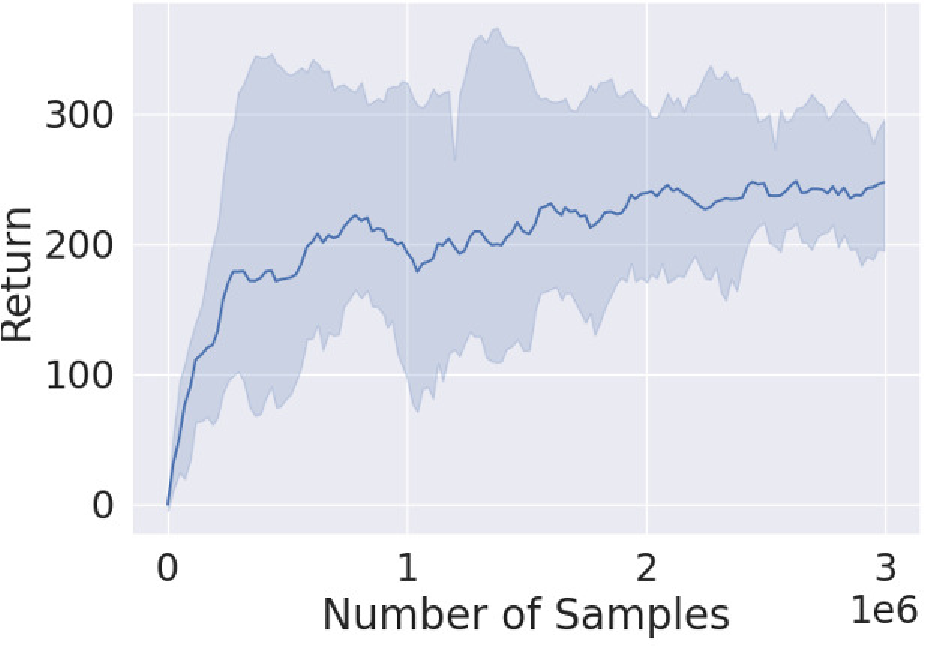
\includegraphics[width=1.5in, height=0.8in]{wk-m-rep-mz.pdf}}
\subfigure[wk-medium]{
\label{fig:1(k)} 
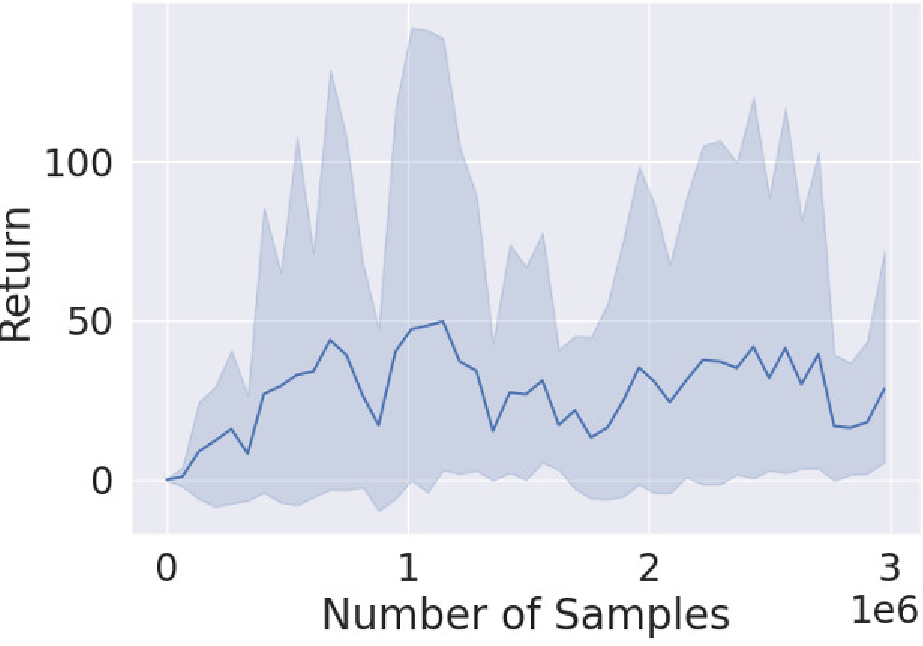
\includegraphics[width=1.5in, height=0.8in]{wk-med-mz.pdf}}
\subfigure[wk-random]{
\label{fig:1(l)} 
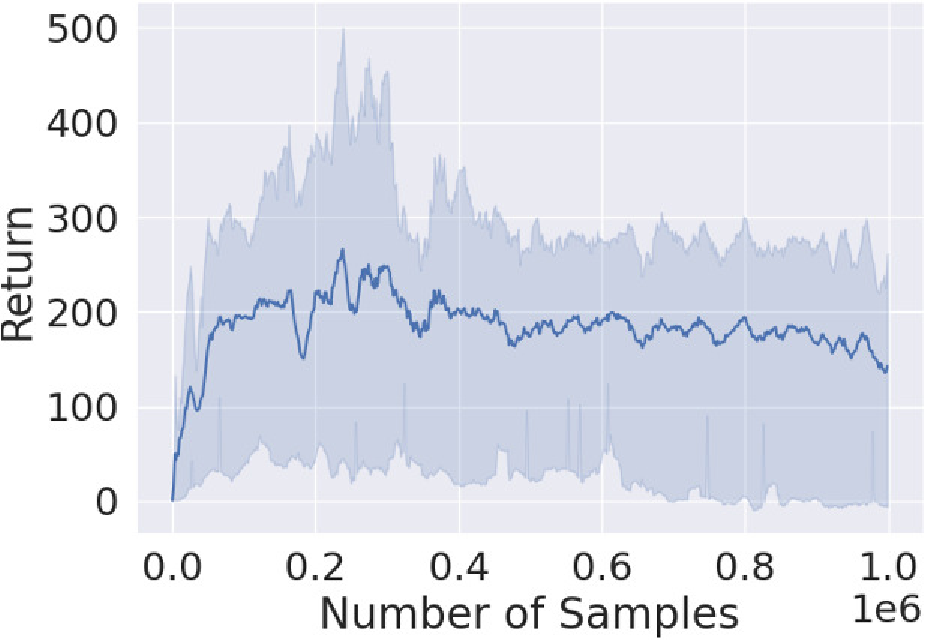
\includegraphics[width=1.5in, height=0.8in]{wk-rnd-mz.pdf}}
\caption{Performance of Sampled EfficientZero on D4RL MuJoCo tasks. The results for HalfCheetah, Hopper, and Walker2d are presented in the three rows, respectively. Each subfigure depicts the change in undiscounted episodic return as a function of the number of training samples. Experiments are repeated three times with different random seeds, with the solid line representing the mean and the shaded area indicating the 95\% confidence interval. For reference, the expert-level episodic returns for HalfCheetah, Hopper, and Walker2d are 12135, 3234.3, and 4592.3, respectively.}
\label{fig:1} 
\end{figure*}


\begin{figure}[t]
    \centering
    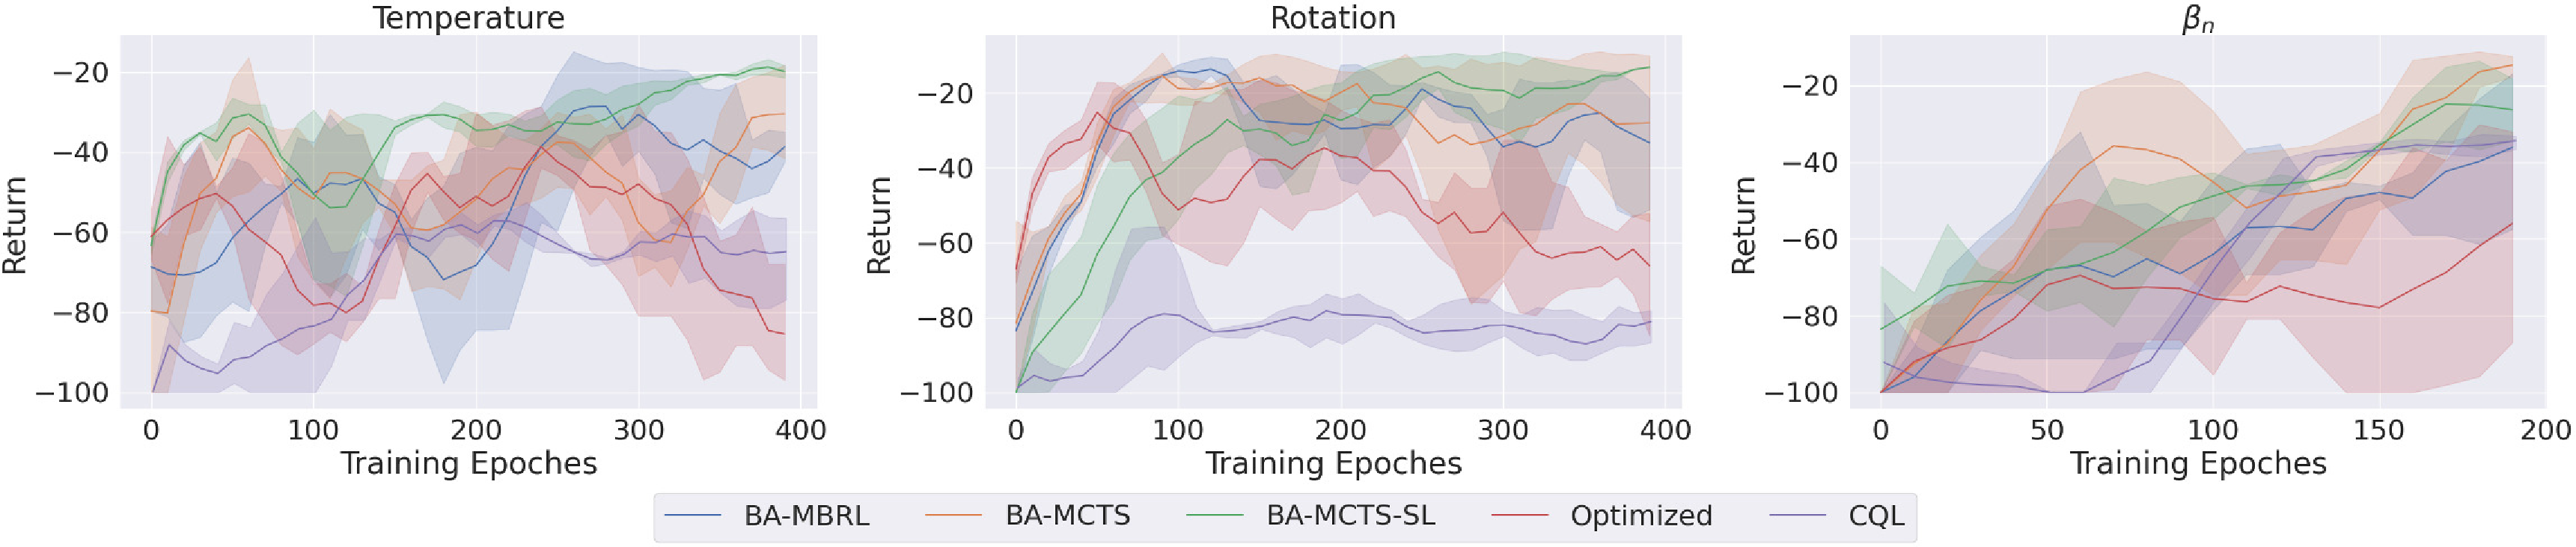
\includegraphics[width=\linewidth, height=1.5in]{nf_return-eps-converted-to.pdf} % or use height
    \caption{Evaluation results for the tokamak control tasks. The figure shows the change in episodic returns over training epochs for the proposed algorithms and baselines across three target tracking tasks in the nuclear fusion scenario. Solid lines represent the average performance, while shaded areas indicate the 95\% confidence intervals.}
    \label{fig:2}
\end{figure}

For fair comparisons and real-time execution, we do not perform test-time search and adopt the same policy architecture as the baselines, i.e., a feedforward neural network, rather than an RNN that incorporates transition history as input. These alternative designs have the potential to further improve our algorithms. For implementation, we build on the codebase of Optimized (\cite{DBLP:conf/iclr/LuBPOR22}), which thoroughly explores design choices in offline MBRL, making minimal changes to the code and hyperparameter settings\footnote{The detailed hyperparameter setups of our algorithms are provided in Appendix \ref{KeyPara}.}. Therefore, we believe the performance improvements stem from the Bayesian RL framework and deep search component. Further, both components can be seamlessly integrated with other advancements in offline MBRL, such as more accurate world model learning and improved uncertainty quantification for constructing pessimistic MDPs. 

MuZero also applies deep search to MBRL. To evaluate its performance on D4RL MuJoCo tasks, we use the open-source implementation and hyperparameter configurations of Sampled EfficientZero (\cite{DBLP:conf/nips/YeLKAG21}) provided by LightZero (\cite{DBLP:conf/nips/NiuPYLZRHLL23}). Benchmarking results from LightZero indicate that Sampled EfficientZero, equipped with a Gaussian policy, achieves the best performance on (online) MuJoCo locomotion tasks compared to other MuZero variants. To adapt Sampled EfficientZero for offline learning, we employ the reanalyse technique proposed by (\cite{DBLP:conf/nips/SchrittwieserHM21}). The evaluation results are presented in Figure \ref{fig:1}. For reference, the expert-level episodic returns (corresponding to scores of 100) for HalfCheetah, Hopper, and Walker2d are 12135, 3234.3, and 4592.3, respectively. As shown, the results are significantly worse compared to the performance of offline RL methods listed in Table \ref{table:1}, despite Sampled EfficientZero's higher computational cost (detailed in Appendix \ref{CompCost}). Notably, both Sampled EfficientZero and BA-MCTS-SL rely on supervised learning for policy improvement. However, for continuous control tasks, the agent can only sample a finite number of actions at a decision point, and the search result (e.g., $\pi_{\text{ret}}$ in Algorithm \ref{alg:2}) is a distribution over this finite set, which could be a poor approximation of the optimal action distribution. Thus, purely mimicking the search result may be less sample-efficient than policy gradient methods, as it fails to account for the continuous nature of the action space. Furthermore, world model learning is the foundation of MBRL and can be particularly challenging in \textbf{continuous control and offline learning settings}, where the state-action space is vast but training data is limited. Sampled EfficientZero integrates model learning and policy training into a single stage, which significantly increases the learning difficulty (compared to BA-MCTS-SL).

Finally, we evaluate our algorithms on three target tracking tasks in tokamak control. The tokamak is one of the most promising confinement devices for achieving controllable nuclear fusion, where the primary challenge lies in confining the plasma, i.e., an ionized gas of hydrogen isotopes, while heating it and increasing its pressure to initiate and sustain fusion reactions (\cite{1512794}). Tokamak control involves applying a series of direct actuators (e.g., neutral beam, ECH power, magnetic field) and indirect actuators (e.g., setting targets for the plasma shape and density) to confine the plasma to achieve a desired state or track a given target. This sophisticated physical process is an ideal test bed for our algorithms. Specifically, we use a well-trained data-driven dynamics model provided by \cite{DBLP:journals/corr/abs-2404-12416} as a ``ground truth" simulator for the nuclear fusion process during evaluation, and generate a dataset containing 725270 transitions using this model for offline RL. We select a reference shot (i.e., an episode of a fusion process) from DIII-D\footnote{DIII-D is a tokamak device located in San Diego, California, operated by General Atomics.}, and use its trajectories of Ion Rotation, Electron Temperature, and $\beta_n$ as targets for three tracking tasks. These are critical quantities in tokamak control, particularly $\beta_n$, which serves as an economic indicator of the efficiency of nuclear fusion. The tracking tasks have a 28-dimensional state space and a 14-dimensional action space, both continuous. Moreover, these tasks are \textbf{highly stochastic}, as the underlying dynamics model is a probabilistic neural network and each state transition is a sample from this model. For details on the simulator, and the design of the state/action spaces and reward functions, please refer to Appendix \ref{DetTCT}. We compare our algorithms with SOTA model-free and model-based offline RL methods, specifically CQL and Optimized. The learning performance on the three tracking tasks is shown in Figure \ref{fig:2}, where the x-axis and y-axis represent the training epochs and (negative) full-shot tracking errors, respectively. Our algorithms consistently outperform the baselines. Notably, the offline dataset does not include the reference shot or any similar, nearby shots. Therefore, restricting the policy to stay close to the behavior policy, as done in model-free methods, can be problematic. Also, learning dynamics models for MBRL is quite challenging in this nuclear fusion scenario. Our algorithms share the same ensemble of dynamics models with ``Optimized" for policy learning, and the comparisons can demonstrate the superiority of Bayesian RL and deep search. Figure \ref{fig:2} has been smoothed for visualization\footnote{The episodic return is plotted every 10 training epochs, with the y-axis representing the average value of a sliding window of length 5.}. We further report the average return over the final 10 training epochs in Table \ref{table:6}, and the conclusions align with those from the D4RL MuJoCo tasks, showing the robustness of our proposed algorithms.

\begin{table}[t]
\small
\centering
\begin{tabular}{c|c|c|c|c|c}
\hline
{Task} & {\makecell{BA-MCTS \\ -SL (ours)}} & {\makecell{BA-MCTS \\ (ours)}} & {\makecell{BA-MBRL \\ (ours)}} & {CQL} & {Optimized}\\
\hline 
\hline
{Temperature} & {\textbf{-21.16} $\pm$ 5.00} & {-23.83 $\pm$ 9.66} & {-29.35 $\pm$ 4.72} & {-59.62 $\pm$ 1.57} & {-83.55 $\pm$ 10.56} \\
{Rotation} & {\textbf{-14.14} $\pm$ 1.88} & {-19.07 $\pm$ 5.85} & {-31.33 $\pm$ 11.54} & {-85.48 $\pm$ 2.72} & {-71.54 $\pm$ 9.88} \\
{$\beta_{n}$} & {-37.03 $\pm$ 17.98} & {\textbf{-18.93} $\pm$ 1.75} & {-23.4 $\pm$ 10.77} & {-36.37 $\pm$ 1.17} & {-57.84 $\pm$ 10.27} \\
\hline
\hline
{Average} & {-24.11} & {\textbf{-20.61}} & {-28.03} & {-60.49} & {-70.98} \\
\hline 
\end{tabular}
\caption{Comparisons between the proposed algorithms and offline RL baselines on the target tracking tasks. For each algorithm, we report the average return of the final ten policy learning epochs and its standard deviation across three different random seeds.}
\label{table:6}
\end{table}

 % get rid of implementation tricks, do minimal changes, see the improvement brought by the search component. 

 % muzero fails, learning dyn and policy at the same stage can be very challenging, especially for complex continuous control tasks
\section{Conclusion}
In this work, we advance the method of {machine unlearning} through a novel viewpoint: model sparsification, achieved by weight pruning. We show in both theory and practice that model sparsity plays a foundational and crucial role in closing the gap between exact unlearning and existing approximate unlearning methods. Inspired by that, we propose two new unlearning paradigms,  `prune first, then unlearn' and `sparsity-aware unlearn', which can significantly improve the efficacy of approximate unlearning. We demonstrate the effectiveness of our findings and proposals in extensive experiments across different unlearning setups. Our study also indicates the presence of \textit{model modularity} traits, such as weight sparsity, that could simplify the process of machine unlearning. This may open up exciting prospects for future research to investigate unlearning patterns within weight or architecture space.





\section{Ethics statement}

This paper explores backdoor attacks that can be inserted through data augmentation. For critical applications such as self driving cars, backdoors inserted by malicious attackers could have serious consequences. Therefore, in this paper we aim to encourage people to inspect their augmentation functions to ensure that any external code is clean.
\section{Reproducibility Statement}

\Cref{section:method:ratio} along with \Cref{fig:wide} show how we are altering the standard Transformer architecture.
The specific tasks we trained our Transformers on are given in \Cref{section:method:datasets} with details on the hyperparameters used for training in \Cref{appendix:tasks}.
The main body of our code can be found at GIT-LINK.



\bibliographystyle{iclr2023_conference}
\bibliography{references}

\newpage
\section*{Appendix}
\appendix
\section{AugMix backdoor algorithm}

\begin{algorithm}
\caption{AugMix backdoor}\label{alg:two}
\SetKwInOut{Input}{input}
\SetKwFunction{gb}{getbatnetbatch}
\SetKwFunction{SGD}{SGD}
\Input{batch $B$, transforms $T$, iterations $n$, surrogate model $M$, loss function $L$}
\texttt{\\}
$w\gets$\text{ random samples from Dirichlet(}$1$\text{) in shape (len(}$B$\text{), len(}$T$))\;
$m\gets$\text{ random samples from Beta(}$\alpha, \alpha$\text{) in shape (len}($T$)\;
\texttt{\\}
$U\gets$ apply BADNET backdoor to $B$\;
$l_u\gets L(M(U$.inputs), $U$.labels)\;
$g_u\gets$ backpropagate gradients from $l_u$ to weights of $M$
\texttt{\\}
\For{$n$ iterations}{
    $V\gets$ apply AugMix to $B$.inputs, using weights $w$[i], $m$[i] for $B$.inputs[i]\;
    $l_v\gets L(M(V$.inputs), $V$.labels)\;
    $g_v\gets$ backpropagate gradients from $l_v$ to weights of $M$\;
    \texttt{\\}
    $E\gets||g_u-g_v||^p$\;
    $g_E\gets$ backpropagate gradients from $E$ to $w$ and $m$\;
    \texttt{\\}
    $w,m\gets$\SGD($[w, m],g_E$)\;
}
\Return{$V$}\;
\end{algorithm}

\section{Datasets}

\textbf{MNIST} The MNIST dataset \citep{mnist} consists of 60000 train images and 10000 test images. Each 28x28 pixel greyscale image displays a single digit between 0 and 9 inclusive. The class of the image is the digit it contains.

\textbf{Omniglot} The Omniglot dataset \citep{omniglot} consists of 1623 classes of handwritten characters from 50 different alphabets, with each class containing 20 samples. We downscale the dataset to 28x28 greyscale images and reduce the number of classes to 50. We split each class into 15 train images and 5 test images.

\textbf{CIFAR-10} The CIFAR-10 dataset \citep{cifar} consists of 50000 train images and 10000 test images, both equally split into 10 classes. Each 32x32 pixel colour image displays a subject from one of the 10 classes.

\textbf{CIFAR-100} The CIFAR-100 dataset \citep{cifar} is similar to the CIFAR-10 dataset, but with 100 classes of 500 train and 100 test images.

\section{Models}

\textbf{ResNet} We use a ResNet-50 classifier for the CIFAR-10 dataset \citep{resnet}, and the WideResNet variant implementation at \href{https://github.com/meliketoy/wide-resnet.pytorch}{https://github.com/meliketoy/wide-resnet.pytorch} to train our CIFAR-100 classifier.

\textbf{DenseNet} We use the DenseNet \citep{densenet} implementation at \href{https://github.com/amurthy1/dagan\_torch}{https://github.com/amurthy1/dagan\_torch} to train our Omniglot classifier.

\textbf{CNN} We use a CNN with two convolutional layers for our MNIST classifiers. The architecture of our classifiers is detailed in Table 4.

\section{Hardware systems}

The testing of our GAN and AugMix backdoors was carried out on a hardware system with 4x NVIDIA GeForce GTX 1080 Ti. The simple transform backdoor training was carried out on NVIDIA T4 GPUs.

% idk what this does but it makes the table go to the top
\makeatletter
\setlength{\@fptop}{0pt}
\makeatother

\begin{table}[ht!]
\caption{Architecture of the classifier we trained on the MNIST dataset}
\centering
\adjustbox{scale=1.0}{\begin{tabular}{c|ccccc}
\hline
& input & filter shape & stride & output & activation \\
\hline
Conv0 & (1, 28, 28) & (8, 1, 5, 5) & 1 & (8, 24, 24) & ReLU \\
Pool0 & (8, 28, 28) & Max, (2, 2) & 2 & (8, 12, 12) & \\
Conv1 & (8, 12, 12) & (16, 8, 5, 5) & 1 & (16, 8, 8) & ReLU \\
Pool1 & (16, 8, 8) & Max, (2, 2) & 2 & (16, 4, 4) & \\
Dense0 & (16, 4, 4) & & & (128) & ReLU \\
Dense1 & (128) & & & (96) & ReLU \\
Dense2 & (96) & & & (10) & \\
\hline
\end{tabular}}
\end{table}


\end{document}
